\documentclass{beamer}
\usepackage[czech]{babel}
\usepackage[utf8]{inputenc}
\usetheme{Boadilla}
\usecolortheme{crane}
\title[Interpret jazyka IFJ11]{Interpret jazyka IFJ11}
\institute{FIT VUT Brno}
\author{~~L. Brabec, R. Mokrá, A. Dujíček, J. Sedlák~~\\}
\date{2011}
\begin{document}

\begin{frame}
  \maketitle
\end{frame}

\begin{frame}
  Tým číslo 097, varianta 1/$\alpha$/I.
  \begin{itemize}
  \item Quicksort
  \item Binární vyhledávací strom
  \item Knuth-Morris-Prattův algoritmus
  \end{itemize}
\end{frame}

\begin{frame}{Obrázek}
  \begin{figure}
    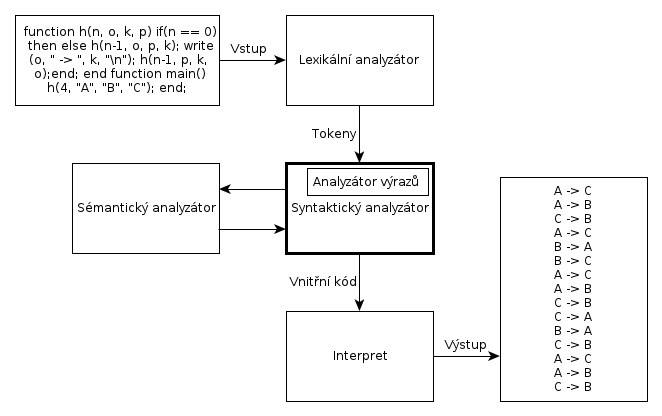
\includegraphics[scale=0.45]{schema.png}
  \end{figure}
\end{frame}

\begin{frame}{Lexikální analýza}
  \begin{figure}
    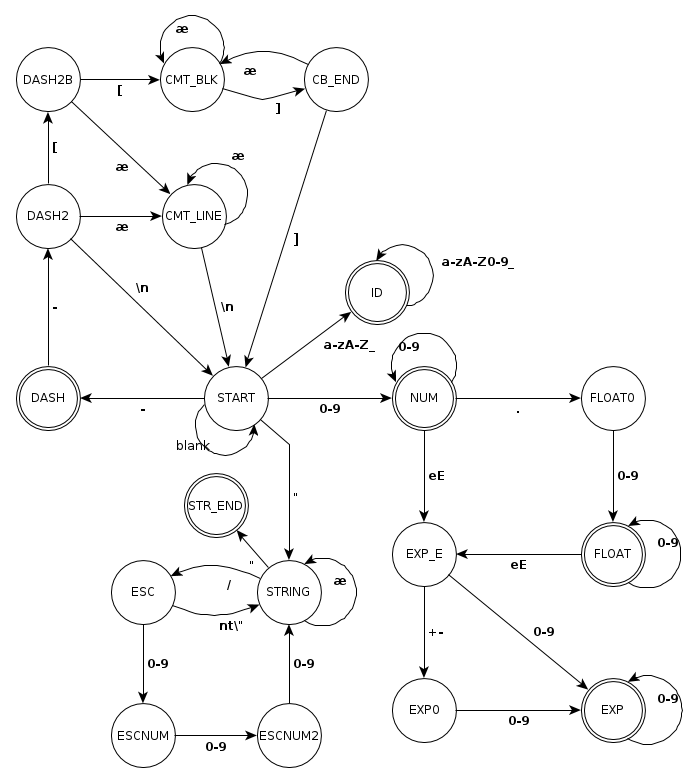
\includegraphics[scale=0.25]{lexical.png}
  \end{figure}
  \begin{itemize}
  \item rozlišení klíčových slov od identifikátorů
  \end{itemize}
\end{frame}

\begin{frame}{Syntaktická analýza}
  \begin{itemize}
  \item metoda rekurzivního sestupu shora dolů
  \item LL-gramatika
  \item výrazy se zpracovávají zvlášť
  \item generují se instrukce
  \item REPEAT
  \item VOIDCALL
  \item LOCALEXPR
  \end{itemize}
\end{frame}

\begin{frame}{Zpracování výrazů}
  \begin{itemize}
  \item zdola nahoru
  \item precedenční tabulka
  \item zpracování argumentů funkcí
  \item FUNEXP
  \end{itemize}
\end{frame}

\begin{frame}{Interpret}
  \begin{itemize}
  \item inspirace x86
  \item zásobníková aritmetika
  \item lokální proměnné na zásobníku
  \end{itemize}
  TODO: nakreslit graf vyuzivani zasobniku
\end{frame}

\begin{frame}{Volání funkcí}
  \tt{function foo(bar, spam, egg)\\\hspace{2em} local x;\\\hspace{2em} return 0;\\end}\\
  \ldots\\
  \tt{foo(2,3);}\\
  \begin{center}
  \begin{tabular}{|c l|}
    \hline
    2 & (bar)\\\hline
    3 & (spam)\\\hline
    nil & (egg)\\\hline
    nil & (x)\\\hline
    0x1ace & (EIP)\\\hline
    456 & (EBP)\\\hline
  \end{tabular}
  \end{center}
\end{frame}

\begin{frame}{}
  Radka Mokrá Vám přeje veselé Vánoce.\\
  Aleš Dujíček Vám děkuje za body.\\
  Jan Sedlák říká: ``Sbohem a dík za všechny ryby.''\\
  Lukáš Brabec mlčky přikyvuje.
\end{frame}

\end{document}
